\subsection{Randlinie} \label{ssec:fahrspurerkennung:riverflow:randlinie}
\subsubsection{Startpunktgewinnung}
Um den eigentlichen Riverflow-Algorithmus ausführen zu können wird die ungefähre Lage der seitlichen Fahrbahnmarkierungen in der Nähe des Fahrzeugs benötigt. Zur Ermittlung dieser gibt es 3 Möglichkeiten:
\begin{enumerate}
\item \label{item:solidline:startpoints:dashedline}
Die Bestimmung durch Orientierung und Position des ersten vor dem Fahzeug gelegenen Mittellinienelementes. Hierzu wird der Mittelpunkt des Elementes senkrecht zu seiner Orientierung um die Fahrspurbreite nach links/rechts verschoben. BILD
\item \label{item:solidline:startpoints:hough}
Eine eindimensionale Hough-Transformation des Bildausschnittes direkt vor dem Fahrzeug wie in \ref{ssec:grundlagen:hough:vereinfachte} beschrieben. BILD
\item \label{item:solidline:startpoints:fixed}
Annahme einer festen Position vor dem Fahrzeug/im Kamerabild.
\end{enumerate}

\begin{figure}[htb]
  \centering
  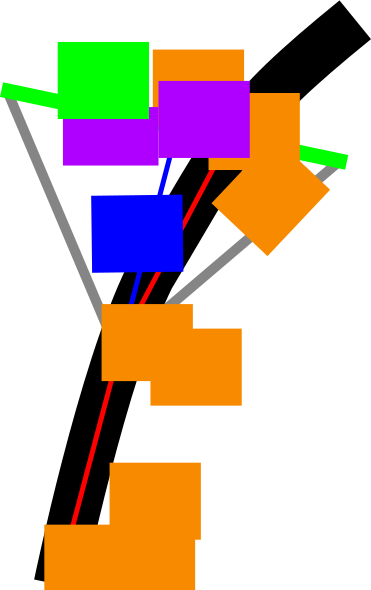
\includegraphics[width=0.5\textwidth]{riverflow_randlinie_prinzip}
  \caption{Funktionsweise des Riverflow-Algorithmus}
  \label{fig:riverflow:randlinie:prinzip}
\end{figure}

\subsubsection{zentraler Algorithmus}
Durch Nutzung der Eigenschaften \ref{item:riverflow:rule:solidline} und  \ref{item:riverflow:rule:curvature} kann ausgehend von der aktuellen Linienorientierung in einem bestimmten Kegel (graue Linien in \ref{fig:riverflow:randlinie:prinzip}), dessen Öffnungswinkel durch die maximale Krümmung der Fahrspur definiert ist, der weitere Verlauf der Fahrbahnmarkierung angenommen werden.
Algorithmisch genutzt wird dieses Wissen durch die Verwendung der aus \ref{ssec:fahrspurerkennung:kalman:messung} bekannten \glspl{glos:scanline}.
Zuerst wird ein Verschiebungsvektor \(\gls{lat:vvrrp}_{\gls{lat:naturalnumber}}\) zwischen vorletztem (\(\gls{lat:prr}_{\gls{lat:naturalnumber}-1}\)) und letztem gefundenen Punkt  (\(\gls{lat:prr}_{\gls{lat:naturalnumber}}\)) der Fahrbahnmarkierung gebildet \eqref{eq:riverflow:solidline:dispvec}. Ausgehend vom letzten gefundenen Punkt der Linie (\(\gls{lat:prr}_{\gls{lat:naturalnumber}}\)) wird selbiger nun um den Vektor \(\gls{lat:vvrrp}_{\gls{lat:naturalnumber}}\) weiterverschoben und bildet den Mittelpunkt  \begin{math} \boldsymbol{m_{n+1}}  \end{math} \(\gls{lat:mrrs}_{\gls{lat:naturalnumber}+1}\) der nächsten \gls{glos:scanline} \eqref{eq:riverflow:solidline:scanlinemidpoint}.
\begin{equation}
\label{eq:riverflow:solidline:dispvec}
\gls{lat:vvrrp}_{\gls{lat:naturalnumber}} =  \gls{lat:prr}_{\gls{lat:naturalnumber}} - \gls{lat:prr}_{\gls{lat:naturalnumber}-1}
= 
\begin{pmatrix}
\gls{lat:vvrrpx} \\
\gls{lat:vvrrpy}
\end{pmatrix}
\end{equation}
\begin{equation}
\label{eq:riverflow:solidline:scanlinemidpoint}
\boldsymbol{m_{n+1}} =  \boldsymbol{p_n} + \boldsymbol{v_n}
\end{equation}
Mithilfe des zu \begin{math} \boldsymbol{v_n} \end{math} \eqref{eq:riverflow:solidline:dispvec} senkrechten Richtungsektors \begin{math} \boldsymbol{d_{n+1}} \end{math} \eqref{eq:riverflow:solidline:scanlinedirectionvec} der \begin{math} (n+1)\end{math}-sten  \gls{glos:scanline} \begin{math} \boldsymbol{s_{n+1}} \end{math} kann selbige wie folgt beschrieben werden:
\begin{equation}
\label{eq:riverflow:solidline:scanlinecontinous}
\boldsymbol{s_{n+1}} =
\boldsymbol{m_{n+1}}  + \alpha \cdot \boldsymbol{d_{n+1}}
\; \alpha \in \mathbb{N}
\end{equation}
\begin{equation}
\label{eq:riverflow:solidline:scanlinedirectionvec}
\boldsymbol{d_{n+1}} =
\begin{pmatrix}
-v_{y_n} \\
v_{x_n}
\end{pmatrix}
\end{equation}
Der Wertebereich des skalaren Faktors \begin{math} \alpha \end{math} gibt hierbei die Ausdehnung der \gls{glos:scanline} um Ihren Mittelpunkt \begin{math} \boldsymbol{m_{n+1}}  \end{math} herum an.
Da die Filterantwort des Kantendetekors durch den Algorithmus zur Erkennung der Mittellinie schon für das gesamte Bild vorliegt, kann zur Erkennung der seitlichen Fahrbahnmarkierung auf selbige zurückgegriffen werden. Hierfür wird die Scanline in eine diskrete Koordinatenserie überführt \ref{eq:riverflow:solidline:scanlinediscrete}, deren Elemente auf ganzzahlige Werte gerundet werden.
\begin{equation}
\label{eq:riverflow:solidline:scanlinediscrete}
\boldsymbol{s_{{n+1}_d}} =
\boldsymbol{m_{n+1}}  + z \cdot \boldsymbol{d_{n+1}} 
\; z \in \mathbb{Z}
\end{equation}
Die durch die Koordinatenserie adressierten Pixel der Filterantwort können nun zur weiteren Verarbeitung in einen Zeilenvektor geschrieben werden. 
 \begin{equation}
 \boldsymbol{f} =
 \begin{pmatrix}
 f_1 & f_2 &  \dots & f_i & \dots & f_n
 \end{pmatrix}
 \end{equation}
Nun wird  \begin{math} \gls{math:max}(\boldsymbol{f})  \end{math} ermittelt. Ist \begin{math} \gls{math:max}(\boldsymbol{f})  \end{math} größer als ein bestimmter Schwellwert \begin{math} s \end{math} , wird der Index \begin{math} i_{max} \end{math} des Maxima in \begin{math} \boldsymbol{f}  \end{math} vorgemerkt. Um eine Linie nicht wiederholt zu finden, muss die in \begin{math} \boldsymbol{f} \end{math} verbleibende, durch dieselbe Markierung verursachte Filterantwort entfernt  werden.
\begin{equation}
f_{i_{max}-\text{Linienbreite}/2}  \dots f_{i_{max}} 
 \dots  f_{i_{max}+\text{Linienbreite}/2} = 0
 \end{equation}
Darauffolgend kann nach weiteren \begin{math} s \end{math} überschreitendenden Einträgen in \begin{math} \boldsymbol{f} \end{math} gesucht und wie mit dem ersten \begin{math} \gls{math:max}(\boldsymbol{f})  \end{math} verfahren werden.
Wird kein ausreichend großes \begin{math} \gls{math:max}(\boldsymbol{f}) \end{math} mehr gefunden, können den gefundenen Indizes \begin{math} i_{max} \end{math} via \eqref{eq:riverflow:solidline:scanlinediscrete} Koordinaten \begin{math} \boldsymbol{p_{n+1}} \end{math} zugeordnet werden GLEICHUNG.
Sind mehrere \begin{math} \boldsymbol{p_{n+1}} \end{math} vorhanden, werden ab diesem Zeitpunkt mehrere Hypothesen einer seitlichen Fahrbahnmarkierung verfolgt.
Jetzt kann die nächste Iteration des Riverflow-Algorithmus mit der Bildung des folgenden Verschiebungsvektors \begin{math} \boldsymbol{v_{n+1}} \end{math} starten.

\subsubsection{Sonderfall 1. und 2. Iteration}
Da in der 1. und 2. Iteration keine Punkte \begin{math} \boldsymbol{p_{n-1}} \end{math} und \begin{math} \boldsymbol{p_n} \end{math}  vorhanden sind, muss der Verschiebungsvektor \begin{math} \boldsymbol{v} \end{math} anderweitig bestimmt werden. 
Wurde der Startpunkt wie in \ref{item:solidline:startpoints:dashedline} beschrieben durch ein Mittellinienelement bestimmt, kann dessen Orientierung als Richtung des Verschiebungsvektors genutzt werden.
In den beiden anderen Fällen \ref{item:solidline:startpoints:hough} und \ref{item:solidline:startpoints:fixed} wird eine konstante Verschiebung in Fahrtrichtung des Fahrzeugs genutzt.

\subsubsection{Ende des Algorithmus}
Der Algorithmus wird beendet, sobald:
\begin{itemize}
\item Der Mittelpunkt \begin{math} \boldsymbol{m}  \end{math} der nächsten Scanline außerhalb des Bildbereichs liegt
\item Auf der aktuellen Scanline keine Maxima größer als der Schwellwert \begin{math} s \end{math} gefunden wurden.
\end{itemize}

\begin{figure}[htb]
  \centering
  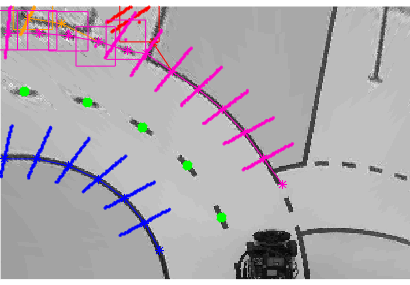
\includegraphics[width=0.75\textwidth]{riverflow_randlinien_komplett}
  \caption{Plot einer eines Riverflow-Durchlaufs für die Randlinien}
  \label{fig:riverflow:randlinien:plot_komplett}
\end{figure}

\subsubsection{Sonderfall gestrichelte Randlinien}
